\documentclass[11pt]{article}

\usepackage{a4wide}
\usepackage{amsmath,amssymb}
\usepackage{color}
\usepackage[utf8]{inputenc}
\usepackage{float}
\usepackage{graphicx}
\usepackage{listings}
\usepackage{multicol}

\newcommand{\code}[1]{{\tt #1}}
\newcommand{\file}[1]{{\tt #1}}

\newcommand{\figref}[1]{(see figure~\ref{#1})}

% usage: \codefig{label}{file}{firstline}{lastline}{description}
\newcommand{\codefig}[5]
{
\begin{figure}[H]
    \lstinputlisting[firstnumber=#3,firstline=#3,lastline=#4]{#2}
    \caption{#5 (#2)}
    \label{code:#1}
\end{figure}
}

\definecolor{comment}{rgb}      {0.38, 0.62, 0.38}
\definecolor{keyword}{rgb}      {0.10, 0.10, 0.81}
\definecolor{identifier}{rgb}   {0.00, 0.00, 0.00}
\definecolor{string}{rgb}       {0.50, 0.50, 0.50}

\lstset
{
    language=matlab,
    % general settings
    numbers=left,
    frame=single,
    basicstyle=\footnotesize\ttfamily,
    tabsize=2,
    breaklines=true,
    showstringspaces=false,
    % syntax highlighting
    commentstyle=\color{comment},
    keywordstyle=\color{keyword},
    identifierstyle=\color{identifier},
    stringstyle=\color{string},
}

\title
{
    {\Large Assignment 1} \\
    Signal \& Image Processing
}

\author
{
    Casper B. Hansen\\
    University of Copenhagen\\
    Department of Computer Science\\
    {\tt fvx507@alumni.ku.dk}
}

\date{\today}

\begin{document}

\maketitle
% \thispagestyle{empty}
% \clearpage


% ASSIGNMENT 1-1
\section{1.1 \mdseries Image generation and manipulation of pixels}
\label{sec:1-1}
In this exercise we are to generate a 20x20 image, show it and take cursor
input, which is then used to manipulate the pixel at that location.

\codefig{1-1}{assignments.m}{7}{19}{Excerpt showing the solution of 1.1}

% TODO: provide description of the program

\begin{multicols}{3}
    
    \begin{figure}[H]
        \center
        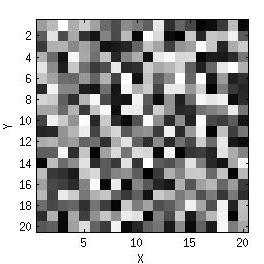
\includegraphics[scale=0.5]{figures/1-1_before.jpg}
        \caption{Before; random generated image}
    \end{figure}
    
    \columnbreak
    
    \begin{figure}[H]
        \center
        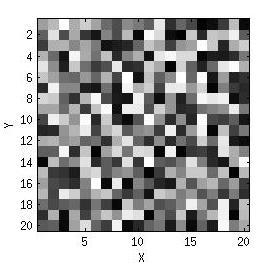
\includegraphics[scale=0.5]{figures/1-1_after.jpg}
        \caption{After; cursor input at $(13,5)$}
    \end{figure}

    \columnbreak
    
    As shown in figure (3), the program work as intended. In the figures
    above, the change is evident at pixel indices $(13,5)$.

\end{multicols}


% ASSIGNMENT 1-2
\section{1.2 \mdseries Display methods}
\label{sec:1-2}
We are to examine the differences in MatLab's methods of displaying
data visually. From {\it Signal Processing Toolbox} we have \code{imshow},
which constrains the proportions of visualizations.

\codefig{1-2}{assignments.m}{21}{28}{Excerpt showing the solution of 1.2}

Unlike \code{imshow}, the generic \code{image}, and quite confusingly, doesn't
interpret the data as an image in the sense of a picture, but rather maps the
matrix data pictorially, and thus does not require proportional constraints.

\begin{figure}[H]
    \center
    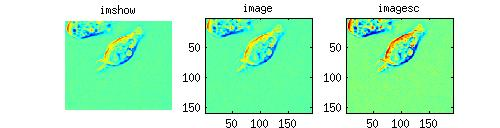
\includegraphics[scale=0.75]{figures/1-2.jpg}
    \caption{Differences in image display functions}
\end{figure}

Lastly, the \code{imagesc} takes the dynamic range of the data, and scales it
to the extremities (minimium and maximum). It allows us to see details that
weren't perceptible beforehand.


% ASSIGNMENT 1-3
\section{1.3 \mdseries Bit-slicing}
\label{sec:1-3}
We are to apply the bit-slicing technique on an arbitrary test image. For this
I've chosen the \file{images/cameraman.tif} picture.

\codefig{1-3}{assignments.m}{30}{38}{Excerpt showing the solution of 1.3}

\begin{multicols}{2}

    As we can see, in figure (7), the first 3 least significant bits doesn't
    contribute much to the picture --- arguably not the fourth either. From
    bit 5 and on, we gradually observe an increase in being able to descern
    objects within the scene, or picture.
    
    Bits 6 and 8 have the highest perceptability in this example.
    
    \vfill\columnbreak

    \begin{figure}[H]
        \center
        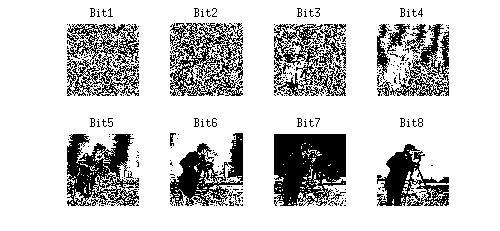
\includegraphics[scale=0.5]{figures/1-3.jpg}
        \caption{Bit-slicing applied to \file{images/cameraman.tif}}
    \end{figure}

\end{multicols}


% ASSIGNMENT 1-4
\section{1.4 \mdseries RGB to HSV conversion}
\label{sec:1-4}
For this assignment, we are to convert an RGB image into HSV colormapping, and
display the changes, as well as its individual channel components.

\codefig{1-4}{assignments.m}{40}{51}{Excerpt showing the solution of 1.4}

In the figure (9) below, we see a clear difference in appearance between the
two formats. The HSV colormap allows us to see details in a picture much
clearer, as it separates much of the visual informations out into separate
channels.

\begin{figure}[H]
    \hspace{-3.5cm}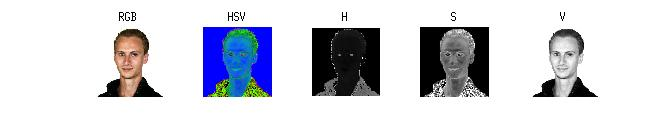
\includegraphics[scale=0.9]{figures/1-4.jpg}
    \caption{HSV converted from RGB, including individual channels}
\end{figure}


% ASSIGNMENT 1-5
\section{1.5 \mdseries Spatial resolution}
\label{sec:1-5}
We are to examine how the digitization process affects the outcome of the
process.

\codefig{1-5}{assignments.m}{53}{73}{Excerpt showing the solution of 1.5}

In figure (10) I present three resizing alterations to an image; a
low-resolution image, a squeezed image (unproportionally scaled), and lastly
an up-scaled image.

\begin{figure}[H]
    \hspace{-3.5cm}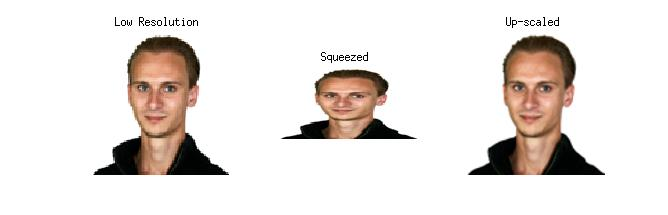
\includegraphics[scale=0.9]{figures/1-5_1.jpg}
    \caption{Image alterations that induces artifacts}
\end{figure}

The loss of detail is quite evident in the low-resolution image (an tenth the
size of the original), and thus appears very {\it pixelated}. The squeezed
image loses much of the vertical detail information, and if stretched back
into proportion would appear somewhat blurred on the vertical axis. Lastly,
the up-scaled image attempts to recreate detail from lost information. In
other words, it must invent pixels by looking at nearby pixels.

To further expand on the notion of {\it inventing pixels}, we examine three
algorithmic techniques for doing so; nearest, bilinear and bicubic.

Each of these algorithms come at an expense to the computation time required
to perform the operation. Therefore their practical application depends on how
fast one must compute the result (ie. real-time applications should generally
be very fast).

\begin{multicols}{3}

    \begin{description}
        \item[Nearest] 6.830 ms
    \end{description}

    \columnbreak

    \begin{description}
        \item[Bilinear] 21.617 ms
    \end{description}

    \columnbreak

    \begin{description}
        \item[Bicubic] 40.825 ms
    \end{description}

\end{multicols}

\begin{figure}[H]
    \hspace{-3.5cm}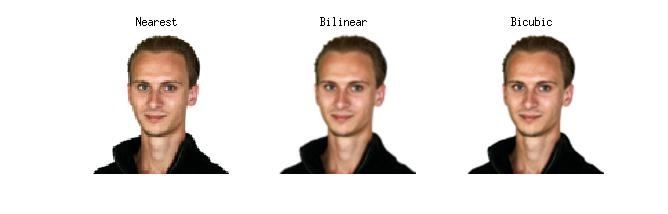
\includegraphics[scale=0.9]{figures/1-5_2.jpg}
    \caption{interpolation algorithms applied to a low-resolution image}
\end{figure}

As we can see, the nearest algorithm is by far the fastest, but also produces
the worst result --- much detail remains lost, and features are obscurred. The
bilinear comes in second and produces a far better image, where most of the
features are preserved well. The last and best, but also the slowest, is the
bicubic algorithm, which preserves much detail and does a very good job at
recreating the original image.


% ASSIGNMENT 1-6
\section{1.6 \mdseries ...}
\label{sec:1-6}
I didn't have time to do this one :(


% assignment 1-7
\newpage
\section{1.7 \mdseries arithmetic operations}
\label{sec:1-7}
We are to examine how arithmetic operations affect the outcome of images.
Also, the assignment asks us to examine resizing of the images to be used,
such that they are of the same size. I found this difficult to understand
however, since the images are already of the same size.

\codefig{1-7}{assignments.m}{80}{89}{Excerpt showing the solution of 1.7}

The $+$ and $-$ operators are, as far as I could tell from the documentation,
equivalent to \code{imadd} and \code{imsubtract} in how they work on basic
appliance --- only special cases give rise to differences, so one set will be
omitted.

\begin{figure}[H]
    \hspace{-1cm}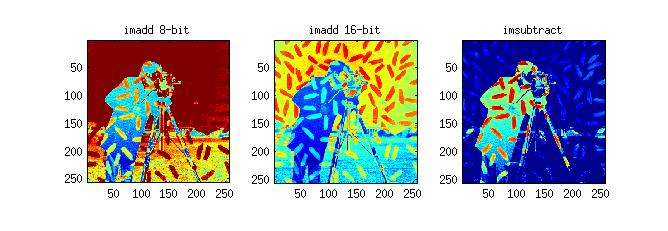
\includegraphics[scale=0.75]{figures/1-7.jpg}
    \caption{Outcomes of arithmetic operations}
\end{figure}

As we can see from figure (14), there is a clear difference in how much detail
is produced by the 16-bit addition operation, compared to that of the 8-bit
addition --- one can clearly descern both pictures in the 16-bit version.


% ASSIGNMENT 1-8
\newpage
\section{1.8 \mdseries Differences across sequences}
\label{sec:1-8}
We use the \code{imabsdiff} function to determine the difference between two
images. Doing so over a sequence of $n$ images produces $n-1$ images.

\codefig{1-8}{assignments.m}{91}{107}{Excerpt showing the solution of 1.8}

\begin{figure}[H]
    \hspace{-3cm}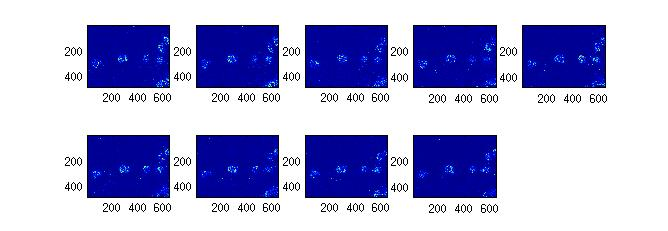
\includegraphics[scale=0.9]{figures/1-8.jpg}
    \caption{Differences over a sequence of 10 images}
\end{figure}


% ASSIGNMENT 1-9
\newpage
\section{1.9 \mdseries Writing functions in MatLab}
\label{sec:1-9}

\begin{multicols}{2}

\codefig{1-9-a}{blend.m}{1}{3}{Excerpt showing the solution of 1.9}

In the code figure below, an example of its application is given.

\codefig{1-9-b}{assignments.m}{109}{115}{Excerpt showing the application of
the solution for 1.9}

\vfill\columnbreak

Writing a function must occur in its own file (here \file{blend.m}), where I
declare it as taking 4 arguments; the two images, and the two weight
coefficients. It performs the weighting element-wise on both images and adds
their respective results to form the returned image.

\begin{figure}[H]
    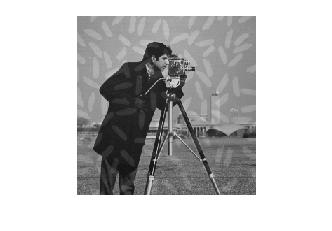
\includegraphics[scale=0.75]{figures/1-9.jpg}
    \caption{Shows the result of code figure (18)}
\end{figure}

\end{multicols}

\end{document}

